\section{Kapazitiver Sensor}
Der Kapazitive Sensor gibt einen Strom, in Abhängigkeit der Distanz zum Objekt, aus. Dieser
Strom generiert einen Spannungsabfall über einen „Bürde-Widerstand“ von 100 Ohm.\\

\subsection{Linearisierung}
Dieses Diagramm zeigt den Mittelwert und die Linearisierung des Kapazitiven Sensors im Bereich von 0 bis 16mm mit einer Schrittweite von 0.5mm.
\begin{figure}[H]
    \centering
    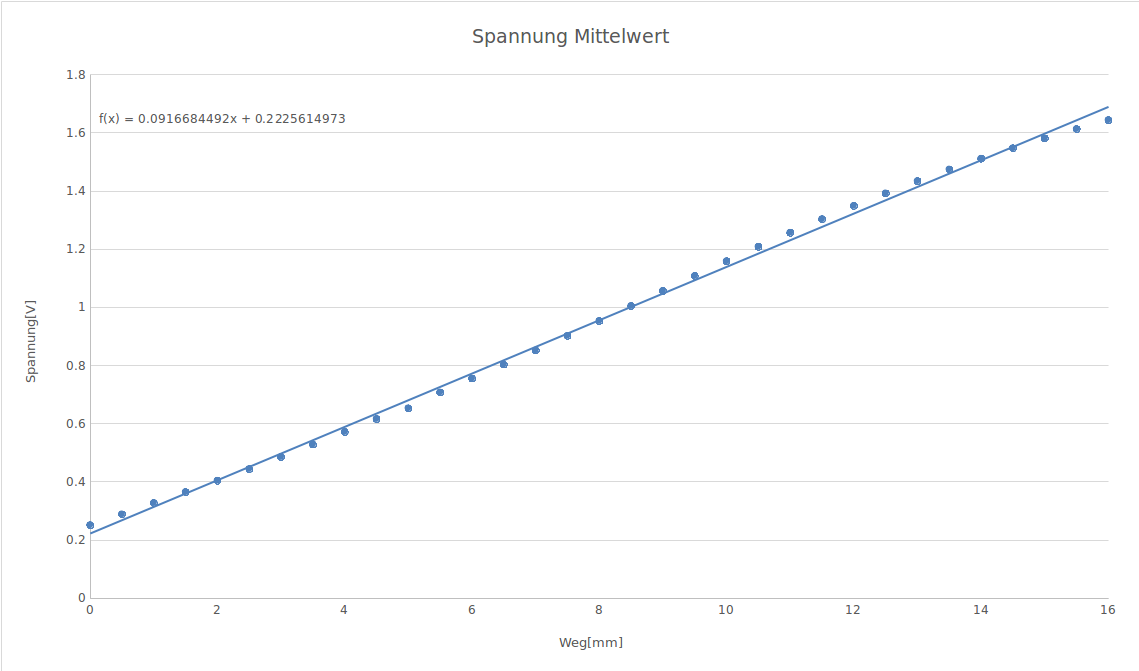
\includegraphics[scale=0.5]{pic/linearisierung.png}
    \caption{Kapazitiven Sensor}
    \label{fig:kapazitiv}
\end{figure}

Die Linearisung wurde anhand der Methode der kleinsten Quadrate vorgenommen. Die Geradengleichung der Linearisierung entspricht: $y = 0.0917x + 0.2228$\\
Diese Gleichung dient zur Rekonstruktion, damit die Spannung des Sensors in eine Distanz umgerechnet werden kann.


\subsection{Hysterese und Nichtlinearität}
Diese zwei Diagramme zeigen die Hysterese und die Nichtlinearität des Kapazitiven Sensors im Bereich von 0 bis 16mm mit einer Schrittweite von 0.5mm.

\begin{figure}[H]
    \centering
    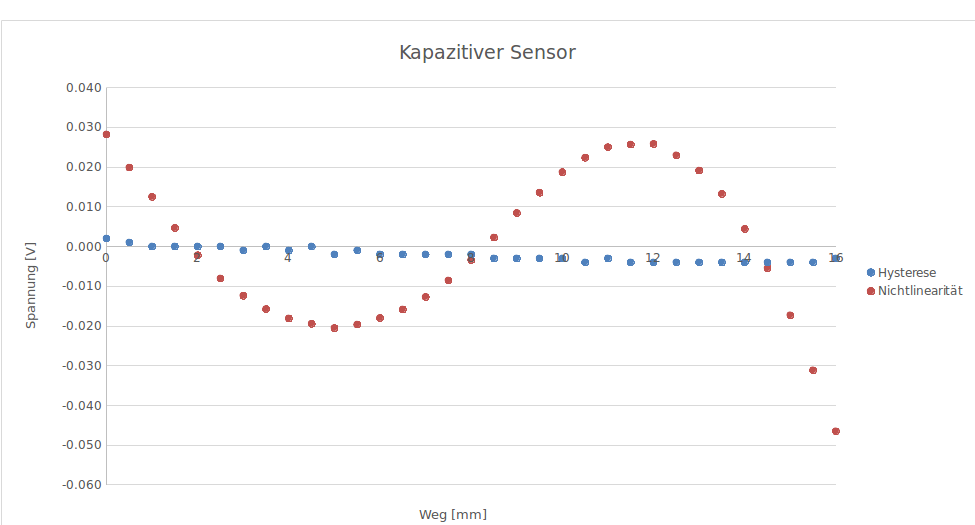
\includegraphics[scale=0.5]{pic/kapazitiv_spannung.png}
    \caption{Kapazitiver Sensor}
    \label{fig:kapazitiv}
\end{figure}


\begin{figure}[H]
    \centering
    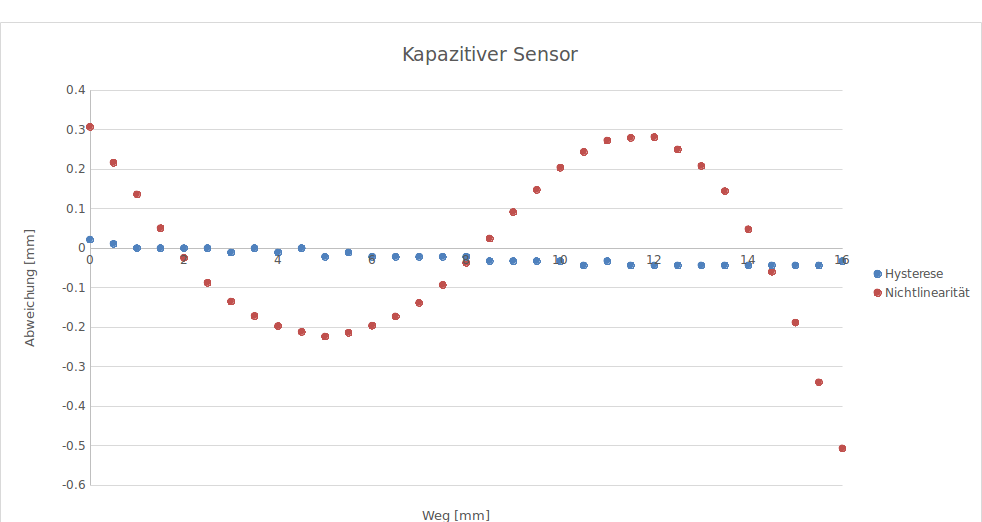
\includegraphics[scale=0.5]{pic/kapazitiv_abweichung.png}
    \caption{Kapazitiver Sensor}
    \label{fig:kapazitiv}
\end{figure}

Die Abweichung in mm ist proportional zur Spannungsabweichung um den Faktor: $\frac{1}{0.0917} \approx 10$.

\subsection{Berechnungen}

\begin{tabular}{ l  l }
    Max. Nicht-linearität: & $\varepsilon_L = \frac{|max(\epsilon_L)|}{|Messbereich|}
                                            = \frac{|0.5mm|}{|16mm|}  
                                            = 3.2\%                             $  \\
    Max. Hysterese:        & $\varepsilon_H = \frac{|max(\epsilon_H)|}{|Messbereich|}
                                            = \frac{|0.45mm|}{|16mm|} 
                                            = 0.27\%                             $  \\
\end{tabular}

\clearpage